\section{表达式引导的 \graph 生成器}
\label{sec:search}

\begin{algorithm}[h]
\caption{\sys 的混合 \graph 生成算法。}
\label{algo:generate}
\footnotesize
\begin{algorithmic}[1]
\Require{具有计算图 $\refgraph$ 的 \lax 程序}
\Ensure{一组 \graphs $\mathcal{S}$}
\State $E_O \gets E(\refgraph)$
\State $\mathcal{S}_0, \mathcal{S} \gets \varnothing$ \label{line:init_prefix}
\State \Call{生成下一个核运算符}{$\func{Inputs}(\refgraph)$}
\ForAll{$G \in \mathcal{S}_0$} \label{line:begin_thread_graph_construct}
\State $\mathcal{S} \gets \mathcal{S} \cup \{\Call{线程图构建}{G}\}$\label{line:end_thread_graph_construct}
\EndFor
\Statex
\Function{生成下一个核运算符}{$\kngraph$}\label{line:begin_kn}
    \State $\mathcal{S}_0 \gets \mathcal{S}_0 \cup \{\kngraph\}$
    \ForAll{核图运算符类型 $t$；输入集 $I$}
        \If{对 $\kngraph$ 中每个 $\vi{op}$，$\func{rank}(I, t) > \func{rank}(\vi{op}.I, \vi{op}.t)$} \label{alg:line:kn_order}
        \If{$t$ 是预定义运算符} \label{line:pre-defined}
          \If{$o := \Call{构建运算符}{\kngraph, I, t}$ 合法}
              \State \Call{生成下一个核运算符}{$\kngraph \cup \{o\}$}
          \EndIf
        \Else
          \Comment{$t$ 是图定义运算符}
          \ForAll{$\vi{gridDims}$；$\vi{forloopDims}$} \label{line:graph-defined}
            \State $\tbgraph \gets \func{TBGraph}(I, \vi{gridDims}, \vi{forloopDims})$
            \State \Call{生成下一个块运算符}{$\kngraph, \tbgraph$}
          \EndFor
        \EndIf
        \EndIf
    \EndFor
\EndFunction \label{line:end_kn}
\Statex
\Function{生成下一个块运算符}{$\kngraph, \tbgraph$} \label{line:begin_tb}
    \If{$\tbgraph$ 中所有共享张量已被消耗}
        \If{$o := \Call{构建运算符}{\kngraph, \tbgraph.I, \tbgraph}$ 合法}
            \State \Call{生成下一个核运算符}{$\kngraph \cup \{o\}$}
        \EndIf
    \EndIf
    \ForAll{块图运算符类型 $t$；输入集 $I$}
        \If{对 $\tbgraph$ 中每个 $\vi{op}$，$\func{rank}(I, t) > \func{rank}(\vi{op}.I, \vi{op}.t)$} \label{alg:line:tb_order}
          \If{$o := \Call{构建运算符}{\tbgraph, I, t}$ 合法}
              \State \Call{生成下一个块运算符}{$\kngraph, \tbgraph \cup \{o\}$}
          \EndIf
        \EndIf
    \EndFor
\EndFunction \label{line:end_tb}
\Statex
\Function{构建运算符}{$\ngraph, I, \vi{attrs}$} \label{line:begin_op}
    \State $E \gets \Call{表达式推导}{E(I), \vi{attrs}}$ \Comment{参见表~\ref{tab:expression}}
    \If{$\Call{子表达式}{E, E_O}$} \Comment{通过抽象表达式剪枝}
    \label{line:expr_check}
    \State $S \gets \ngraph.\func{outputTensorShapeInfr}(I, \vi{attrs})$
    \Comment{检查张量形状} \label{line:tensor_shape_check}
    \If{$S.\func{valid}$，$\ngraph.\func{mAlloc}+S.\func{size} \le \ngraph.\func{mLimit}$}
        \Comment{检查内存} \label{line:memory_check}
            \State \Return $\ngraph.\func{constructOp}(I, \vi{attrs})$
        \EndIf
    \EndIf
    \State \Return 非法
\EndFunction \label{line:end_op}
\Statex
\Function{线程图构建}{$G$}
    \State $\GF{fused} \gets G$
    \While{$\exists o \in \GF{fused}$ 可与其前驱运算符融合}
        \State $\GF{fused} \gets \Call{融合运算符}{\GF{fused}, o}$
    \EndWhile
    \State \Return $\GF{fused}$
\EndFunction

\end{algorithmic}
\end{algorithm}

本节介绍 \sys 的 \graph 生成器，它能自动为输入张量程序发现潜在的 \graphs。
为了生成能够捕获核、块和线程层次优化的 \graphs，\sys 必须探索比现有超级优化器大得多的搜索空间，现有超级优化器只考虑核层次的优化。
\sys 采用两项关键技术来应对这一挑战。
第一，基于核和块层次的优化对性能的影响远比线程层次更为关键这一观察——因为访问设备内存和共享内存比访问寄存器文件昂贵几个数量级——\sys 的 \graph 生成器采用了一种{\em 混合方法}：在核和块层次穷举考虑所有不超过一定大小的可能图，并使用基于规则的策略来构建线程层次的图。这一方法在保留大多数性能关键优化的同时缩减了搜索空间。
第二，为了进一步剪枝搜索空间，\sys 引入了一种基于 \graphs 抽象的剪枝技术，称为{\em 抽象表达式}，在提供一定理论最优性保证的同时减少了 \sys 需要考察的 \graphs 数量。
我们在 \S\ref{subsec:kernel_block_graph_generation} 和 \S\ref{subsec:thread_graph_construction} 中介绍混合 \graph 生成算法，在 \S\ref{subsec:abstract_expression} 中介绍表达式引导的剪枝技术。

\subsection{核图和块图生成}
\label{subsec:kernel_block_graph_generation}
\sys 增量式地生成核图和块图，并利用多种剪枝技术来缩减搜索空间，如 \Cref{fig:generator} 第二部分所示。
具体来说，\sys 维护一个合法 \graph 的{\em \prefix}，并通过迭代方式用新运算符扩展它。
对于图 $G=(V,E)$，若其子图 $G'=(V',E')$ 满足 $\forall u \in V', \forall (v, u) \in E, v \in V'$，则称 $G'$ 为 $G$ 的一个{\em 前缀}。

为了生成核图中的下一个运算符，\sys 枚举核运算符类型 $t$ 和输入张量集 $I$。若 $t$ 表示图定义运算符类型，\sys 将通过（1）枚举网格维度和 for 循环维度（见 \S\ref{sec:hcg}），计算块图的输入张量形状；以及（2）执行与核层次类似但不考虑图定义运算符的嵌套生成过程，来生成定义其核计算的关联块图。\Cref{algo:generate} 中的第 \ref{line:begin_kn}--\ref{line:end_kn} 行和第 \ref{line:begin_tb}--\ref{line:end_tb} 行分别展示了 \sys 如何生成核运算符和块运算符。

\sys 在添加运算符之前检查张量形状（第 \ref{line:tensor_shape_check} 行）和内存使用（第 \ref{line:memory_check} 行），以确保前缀合法。

为了确保相同的 \graphs 只被生成一次，\sys 定义了 \graphs 的{\em 标准形式}。
对于一个算子按拓扑顺序为 $o_1, \ldots, o_n$ 的 \graph $G$，$o_i$ 的第 $j$ 个输出的{\em 索引}定义为元组 $(i, j)$。$G$ 中每个运算符 $o_i$ 被赋予一个{\em 秩}（rank）$(\vi{input}_i, \vi{type}_i)$，其中 $\vi{input}_i$ 是 $o_i$ 输入张量索引的列表，$\vi{type}_i$ 是运算符类型。
若 \graph 的运算符按秩递增排列，则称其处于标准形式。
\sys 通过要求运算符按秩递增顺序添加（第 \ref{alg:line:kn_order} 行和第 \ref{alg:line:tb_order} 行）来只生成标准形式的 \graphs。这种方法不会剪枝掉任何有效解，因为每个 \graph 都可以通过重排运算符的顺序转换为标准形式。

此外，\sys 利用{\em 抽象表达式}技术来剪枝不满足特定约束的前缀，这将在 \S\ref{subsec:abstract_expression} 中介绍。

\subsection{线程图构建}
\label{subsec:thread_graph_construction}

尽管类似的嵌套生成策略也可以应用于线程图，但 \sys 选择使用基于变换的方法来构建线程图（见 \Cref{fig:generator} 第三个面板以及 \Cref{algo:generate} 中的第 \ref{line:begin_thread_graph_construct}--\ref{line:end_thread_graph_construct} 行），以缩减搜索空间。

\sys 在构建线程图时应用运算符融合，通过尽可能在寄存器文件中重用张量来减少对共享内存的访问。
例如，\sys 将 \Cref{fig:rms_norm_mlso} 中的三个逐元素运算符（{\tt Mul}、{\tt Sqrt} 和 {\tt Div}）融合到一个线程图中，避免将中间结果保存到共享内存，并将这些运算符的整个计算保持在寄存器文件中。
虽然我们目前的实现侧重于运算符融合，但也可以使用额外的基于规则的变换来构建线程图。

\begin{table}
    \centering
    \caption{\sys 支持的运算符。第二列显示支持该运算符的图层次（K、B 和 T 分别表示核图、块图和线程图）。最后一列定义每个运算符输出的抽象表达式，其中 $E$ 将张量映射到其抽象表达式。}
    \vspace{\captionvspace}
    \label{tab:expression}
    \resizebox{\columnwidth}{!}
    {%
    \begin{threeparttable}
    \begin{tabular}{l|l|l}
    \toprule
    {\bf \graph 运算符} & {\bf 图层次} &  {\bf 输出张量的抽象表达式} \\
    \midrule
    InIter & B & $\expr(\mathrm{InIter}(X)) = \expr(X)$ \\
    OutSaver  & B & $\expr(\mathrm{OutSaver}(X)) = \expr(X)$ \\
    Matmul & K, B, T & $\expr(\mathrm{Matmul}(X, Y)) = \ered(k, \emul(\expr(X), \expr(Y)))$\tnote{1} \\
    Sum & K, B, T & $\expr(\mathrm{Sum}(d_r, k_r, X)) = \ered(k_r, \expr(X))$\tnote{2} \\
    EwAdd & K, B, T & $\expr(\mathrm{EwAdd}(X, Y)) = \eadd(\expr(X), \expr(Y))$ \\
    EwMul & K, B, T & $\expr(\mathrm{EwMul}(X, Y)) = \emul(\expr(X), \expr(Y))$ \\
    EwDiv & K, B, T & $\expr(\mathrm{EwDiv}(X, Y)) = \ediv(\expr(X), \expr(Y))$ \\
    EwExp & K, B, T & $\expr(\mathrm{EwExp}(X)) = \eexp(\expr(X))$ \\
    Repeat & K, B & $\expr(\mathrm{Repeat}(X)) = \expr(X)$ \\
    Reshape & K, B & $\expr(\mathrm{Reshape}(X)) = \expr(X)$ \\
    Sqr & K, B & $\expr(\mathrm{Sqr}(X)) = \emul(\expr(X), \expr(X))$ \\
    Sqrt & K, B & $\expr(\mathrm{Sqrt}(X)) = \esqrt(\expr(X))$ \\
    SiLU & K, B & $\expr(\mathrm{SiLU}(X)) = \esilu(\expr(X))$ \\
    Accum & B & $\expr(\mathrm{Accum}(X, m, i)) = \ered(i, \expr(X))$（若 $m = \phi$，否则 $\expr(X)$）\tnote{3} \\
    \bottomrule
    \end{tabular}
    \begin{tablenotes}
    \item[1] $k$ 表示 $A$ 最后一维（即规约维度）的大小。Matmul 在最内两个维度上执行，前导维度进行批处理。
    \item[2] 沿维度 $d_r$ 对每 $k_r$ 个元素求和。
    \item[3] 沿 fmap $m$ 累积 $i$ 次 for 循环迭代的结果。
    \end{tablenotes}
    \end{threeparttable}
    }
    \vspace{\captionvspace}
\end{table}

\subsection{通过抽象表达式剪枝}
\label{subsec:abstract_expression}

在搜索可能的 \graphs 空间时，我们的目标是避免其中间结果无法对目标计算作出贡献的 \graph 前缀。
例如，对于输入程序 $X \cdot Z + Y \cdot Z$，我们可以剪枝掉计算 $X \cdot Y$ 的前缀，但不应剪枝计算 $X + Y$ 的前缀，因为 $(X+Y) \cdot Z$ 与输入程序等价。
然而，在搜索某个计算的同时，我们如何确定一个前缀是否能对该计算作出贡献呢？
下面，我们通过{\em 抽象化}来绕开这个"先有鸡还是先有蛋"的问题，开发出一种由这一直觉驱动的剪枝技术。
我们首先介绍抽象化方法——{\em 抽象表达式}——然后解释它如何用于剪枝。
最后，我们在特定条件下提供该剪枝不会排除最优 \graph 的理论保证。

\paragraph{抽象表达式。}
回顾一下，\graph 中的一条边对应于输入张量的一个张量值函数。直观地，抽象表达式通过忽略同一输入张量的元素之间的差异来对这些函数进行抽象。
形式上，抽象表达式是整数理论和未解释函数理论上的一阶逻辑项。
在 \graph 中，每条边的抽象表达式（记为 $\expr(\cdot)$）在 \Cref{tab:expression} 中定义。
在计算 \graph 的抽象表达式时，所有图定义运算符都被"内联"处理。
具体来说，为图定义运算符输入计算的表达式被传入其底层图，该底层图的输出表达式即成为图定义运算符的输出表达式。
\Cref{fig:abstract_expression} 展示了注意力计算的一个子图中的抽象表达式。

\begin{figure}
    \centering
    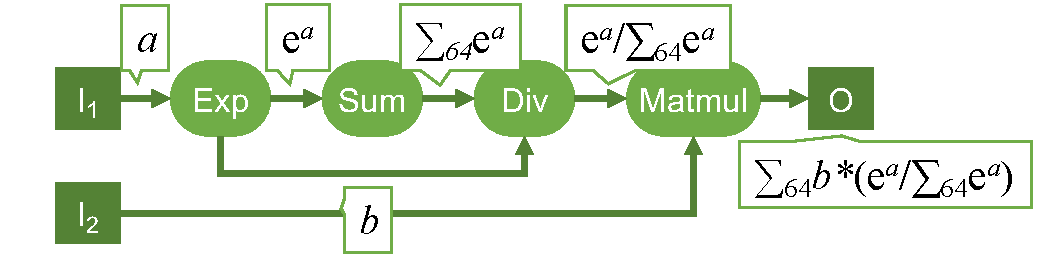
\includegraphics[width=0.9\columnwidth]{figs/expr.pdf}
    \vspace{\captionvspace}
    \caption{抽象表达式示意图。张量的抽象表达式标注在边上。这里使用便于理解的记法：$\mathrm{e}^a$ 表示 $\eexp(a)$，$\sum_k a$ 表示 $\ered(k, a)$，$a/b$ 表示 $\ediv(a, b)$，$a*b$ 表示 $\emul(a, b)$。张量 $I_1$、$I_2$ 和 $O$ 均为 $64\times64$ 矩阵。}
    \vspace{\captionvspace}
    \label{fig:abstract_expression}
\end{figure}

\paragraph{抽象子表达式与剪枝。}
我们使用抽象表达式，通过形式化两种关系——等价关系和抽象子表达式关系——来剪枝 \graphs 的搜索空间。具体地，我们剪枝掉任何抽象表达式不是与输入程序的某个等价抽象表达式的子表达式的 \graph 前缀。

我们将抽象表达式形式化为整数算术理论和未解释函数理论上的一阶逻辑中的未解释函数，并使用 SMT 求解器基于 \Cref{tab:axioms} 中的两组公理 $\Aeq$ 和 $\Asub$ 对其进行推理。

第一，$\Aeq$ 公理化了抽象表达式之间的等价关系。
需要注意的是，这些公理不必是可靠的——并不要求具有等价抽象表达式的 \graphs 在功能上也等价，因为不等价的 \graphs 可能具有相同的抽象表达式。
第二，$\Asub$ 公理化了抽象表达式之间的子表达式关系。$\Asub$ 的一个关键性质是：对于任何 \graph $G_1$ 是 $G_2$ 的前缀——即 $G_2$ 可以通过用额外的运算符扩展 $G_1$ 来构建——有 $\expr(G_1)$ 是 $\expr(G_2)$ 的抽象子表达式；形式上，$\Asub \models \subexpr(\expr(G_1), \expr(G_2))$，其中 $\models$ 表示在整数算术和未解释函数理论下的蕴含。

在搜索过程中，\Cref{algo:generate} 首先计算输入 \lax 程序的抽象表达式（记为 $E_O$），并在 $\Aeq \cup \Asub \not\models \subexpr(\expr(G),E_O)$ 时剪枝任何 \graph 前缀 $G$。即，若一个图的抽象表达式不是 $E_O$ 的子表达式，则将其剪枝。这一检查通过 SMT 求解器（Z3~\cite{z3}）执行。
作为优化，这些检查的结果会被缓存以供复用，因为 \sys 在搜索过程中可能遇到具有相同抽象表达式的多个 \graphs。

\begin{table}[h]
    \centering
    \caption{用于剪枝的抽象表达式公理化。\sys 通过查询 SMT 求解器检验 $\subexpr(E_1, E_2)$ 是否被这些公理蕴含，来判断抽象表达式 $E_1$ 是否为 $E_2$ 的子表达式。所有公理中的变量均全称量化。}
    \vspace{\captionvspace}
    \label{tab:axioms}
    \resizebox{\columnwidth}{!}{
    \begin{tabular}{l|l}
    \toprule
    {\bf 抽象表达式性质} & {\bf 说明} \\
    \midrule
    \multicolumn{2}{l}{\it 等价公理 $\Aeq$} \\
    \midrule
    $\forall x,y.\ \eadd(x, y) = \eadd(y, x)$ & 交换律 \\
    $\forall x,y.\ \emul(x, y) = \emul(y, x)$ & 交换律 \\
    $\forall x,y,z.\ \eadd(x, \eadd(y, z)) = \eadd(\eadd(x, y), z)$ & 结合律 \\
    $\forall x,y,z.\ \emul(x, \emul(y, z)) = \emul(\emul(x, y), z)$ & 结合律 \\
    $\forall x,y,z.\ \eadd(\emul(x, z), \emul(y, z)) = \emul(\eadd(x, y), z)$ & 分配律 \\
    $\forall x,y,z.\ \eadd(\ediv(x, z), \ediv(y, z)) = \ediv(\eadd(x, y), z)$ & 结合律 \\
    $\forall x,y,z.\ \emul(x, \ediv(y, z)) = \ediv(\emul(x, y), z)$ & 结合律 \\
    $\forall x,y,z.\ \ediv(\ediv(x, y), z) = \ediv(x, \emul(y, z))$ & 结合律 \\
    $\forall x.\ x = \ered(1, x)$ & 恒等规约 \\
    $\forall x,i,j.\ \ered(i, \ered(j, x)) = \ered(i*j, x)$ & 结合律 \\
    $\forall x,y,i.\ \ered(i, \eadd(x, y)) = \eadd(\ered(i, x), \ered(i, y))$ & 结合律 \\
    $\forall x,y,i.\ \ered(i, \emul(x, y)) = \emul(\ered(i, x), y) $ & 分配律 \\
    $\forall x,y,i.\ \ered(i, \ediv(x, y)) = \ediv(\ered(i, x), y) $ & 分配律 \\
    $\forall x,y.\ \emul(\eexp(x), \eexp(y)) = \eexp(\eadd(x, y))$ & 分配律 \\
    $\forall x,y.\ \emul(\esqrt(x), \esqrt(y)) = \esqrt(\emul(x, y))$ & 分配律 \\
    
    \midrule
    \multicolumn{2}{l}{\it 子表达式公理 $\Asub$} \\
    \midrule
    $\forall x,y.\ \subexpr(x, \eadd(x, y))$ & \\
    $\forall x,y.\ \subexpr(x, \emul(x, y))$ & \\
    $\forall x,y.\ \subexpr(x, \ediv(x, y))$ & \\
    $\forall x,y.\ \subexpr(y, \ediv(x, y))$ & \\
    $\forall x.\ \subexpr(x, \eexp(x))$ & \\
    $\forall x.\ \subexpr(x, \esqrt(x))$ & \\
    $\forall x.\ \subexpr(x, \esilu(x))$ & \\
    $\forall x,i.\ \subexpr(x, \ered(i, x))$ & \\
    $\forall x.\ \subexpr(x, x)$ & 自反性 \\
    $\forall x,y,z.\ \subexpr(x,y) \wedge \subexpr(y,z) \to \subexpr(x, z)$ & 传递性 \\
    \bottomrule
    \end{tabular}
    }
    \vspace{\captionvspace}
\end{table}

\paragraph{理论保证与剪枝-最优性权衡。}
直观地，我们的剪枝方法会保留所有可能引出其抽象表达式（根据 $\Aeq$）与输入 \lax 程序等价的 \graph 的前缀。形式上：

\begin{theorem}[通过抽象表达式剪枝]
\label{thm:pruning}
对于输入 \graph $G_0$，以及与 $G_0$ 等价的 \graph $G$，
若 $\Aeq \models E(G_0) = E(G)$，则 $G$ 将被 \Cref{algo:generate} 生成。
\end{theorem}

\begin{proof}
由 \Cref{tab:expression,tab:axioms}，我们证明对于任意运算符 $\er{op}$，若 $Y = \er{op}(X_1,\ldots,X_n)$，则对 $1 \leq i \leq n$ 有 $\Asub \models \subexpr(\expr(X_i), \expr(Y))$。
即，$\er{op}$ 每个输入的抽象表达式始终是 $\er{op}$ 输出的子表达式。
考虑到 $\Asub$ 包含自反性和传递性公理，
对于任何 $G'$ 是 $G$ 的前缀，有 $\Asub \models \subexpr(\expr(G'),\expr(G))$。
结合 $\Aeq \models E(G_0) = E(G)$ 的假设，
得到 $\Aeq \cup \Asub \models \subexpr(\expr(G'),\expr(G_0))$。
因此，$G$ 的所有前缀都不会被剪枝，\sys 将生成 $G$。
\end{proof}
